\documentclass[a4paper,12pt]{article}
\usepackage[utf8]{inputenc}
\usepackage{polski}
\author{Marcin Fabrykowski}
\title{Eksploracja danych\\Projekt}
\usepackage{listings}
\usepackage{graphicx}
\begin{document}
\maketitle
\newpage
\tableofcontents
\newpage
\section{Opis problemu}
Celem projektu jest opracowanie klasyfikatora drzewiastego do klasyfikacji wina na podstawie jego parametrów.\\
Jako zbiór do nauki, został wykorzystany zbiór\\
http://archive.ics.uci.edu/ml/datasets/Wine+Quality
\section{Opis etapu przygotowania danych}
Dane źródłowe zamieszczone na stronie internetowej były zapisane w formacie CVS (załączony plik winequality-white.csv\_orig).\\
Plik wejściowy musiał zostać przekonwertowany na format możliwy do wczytania przez bibliotekę Orange.\\
Należało zastąpić separator ';' tabulatorem separującym, oraz usunąć cudzysłowia z z nagłówkowego wiersza.\\
Efekt konwersji jest widoczny w pliku: winequality-white.csv
\section{Klasyfikator}
Klasyfikator jest operatorem potrafiącym, po wcześniejszym 'nauczeniu', przewidzieć klasyfikowaną wartość na podstawie badanych atrybutów. W naszym przypadku wartością klasyfikowaną jest jakość wina.\\
Podczas tworzenia klasyfikatora, mamy możliwość określenia maksymalnej głębokości drzewa (max\_depth) oraz ilości iteracji przycinania drzewa (m\_prning).
\section{Wykorzystywane technologie}
Projekt został napisany w języku Python.\\
Do działania, wymagane są następujące biblioteki:
\begin{itemize}
\item SciPy
\item Orange
\item pygraphviz
\end{itemize}
Orange jest biblioteką wspomagającą operacje związane z eksploracją danych. Udostępnia ona narzędzie do przeprowadzania klasyfikacji, regresji, asocjacji oraz kategoryzacji. Orange pozwala na wyeksportowanie danych o drzewach w formacie .dot, które mogą zostać sparsowane przez program graphviz.
Pygraphviz jest bindingiem do graphviza i pozwala na generowanie diagramów z plików .dot.
\section{Działanie programu}
Na początku następuje sprawdzenie czy w systemie znajdują się wymagane moduły oraz załadowanie ich.\\
Następnie następuje wczytanie danych wejściowych z pliku csv do tabeli systemu Orange.\\
Po wczytaniu danych, następuje wygenerowanie klasyfikatora dla wczytanych danych oraz ustawionych parametrów tego klasyfikatora.\\
Mając wygenerowanie drzewo klasyfikujące, zapisujemy je do pliku w formacie .dot.\\
Wygenerowany plik .dot zostaje przetworzony przez moduł pygraphviz w celu wygenerowanie pliku graficznego PNG przedstawiającego otrzymamy klasyfikator.\\
W ostatnim kroku obliczamy statystyki dla naszego klasyfikatora
\section{Prezentacja wyników}
Wynikiem działania programu jest klasyfikator drzewiasty przedstawiony na rys \ref{fig:klasyfikator}.
\begin{figure}
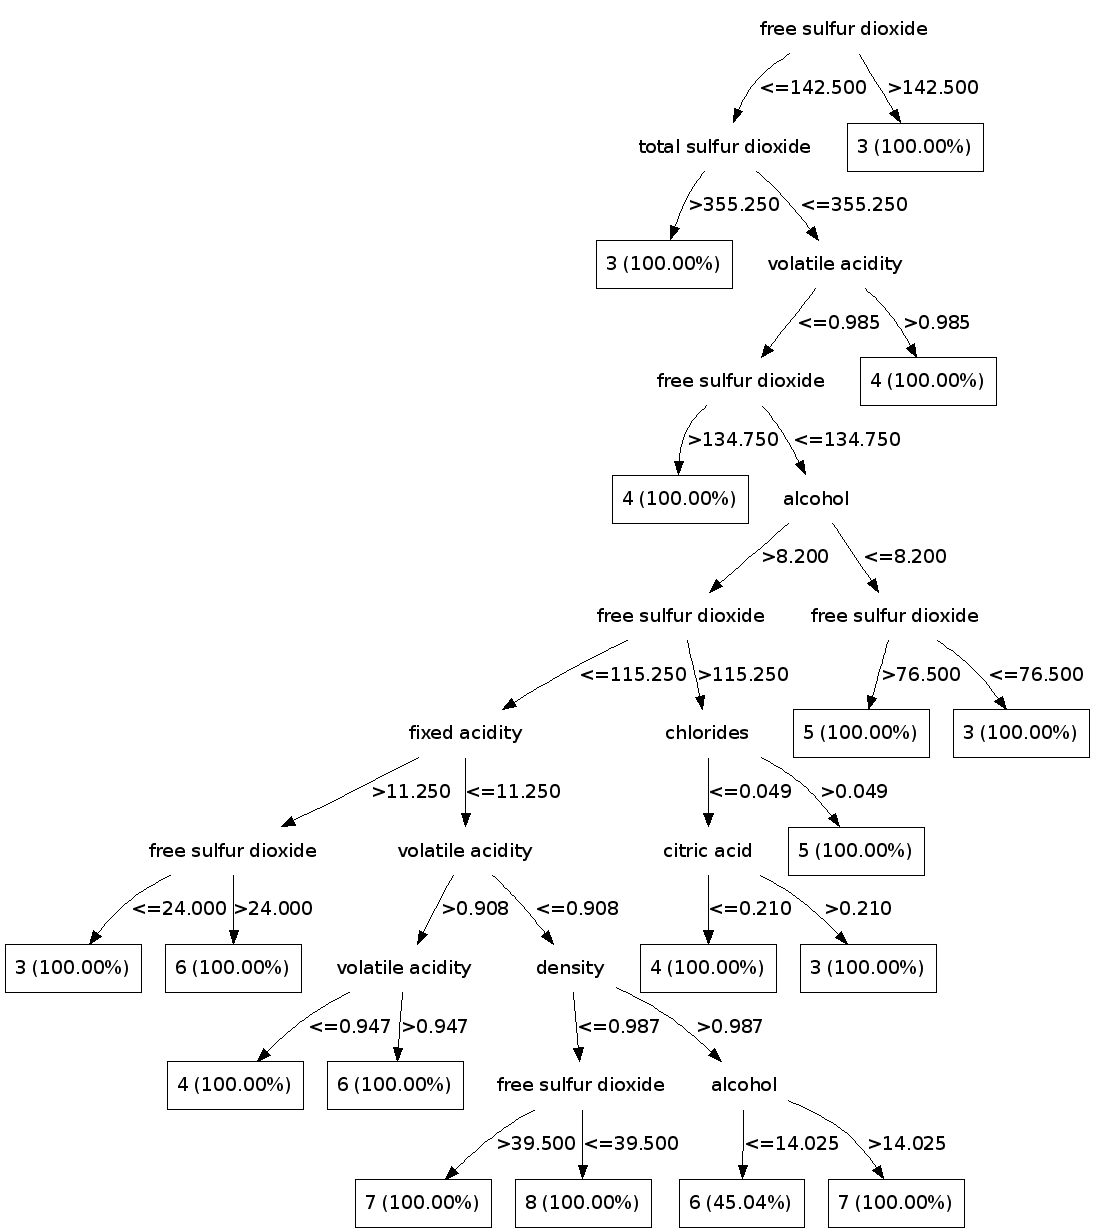
\includegraphics[width=15cm]{FabrykowskiMarcin.png}
\caption{Reprezentacja graficzna klasyfikatora}
\label{fig:klasyfikator}
\end{figure}
\end{document}
